\chapter{Introduction}

The U.S. agricultural industry has long been a cornerstone of the country's economy, contributing over a trillion dollars in value-added to the GDP annually. Specifically, farms generate approximately \$164.7 billion annually, as illustrated in Fig \ref{fig:1.1} \cite{zahniser_kassel_2023, depietro_2022}. One of the significant challenges farmers face is managing pests and crops, with the average cost being approximately ``34\% of a farmer's variable crop production costs" \cite{lrichmond_2007}. While pests can cause economic loss and harm to farmland, there are also beneficial insect species that save growers millions of dollars annually \cite{state_2010}.

\begin{figure}[H]
\begin{center}
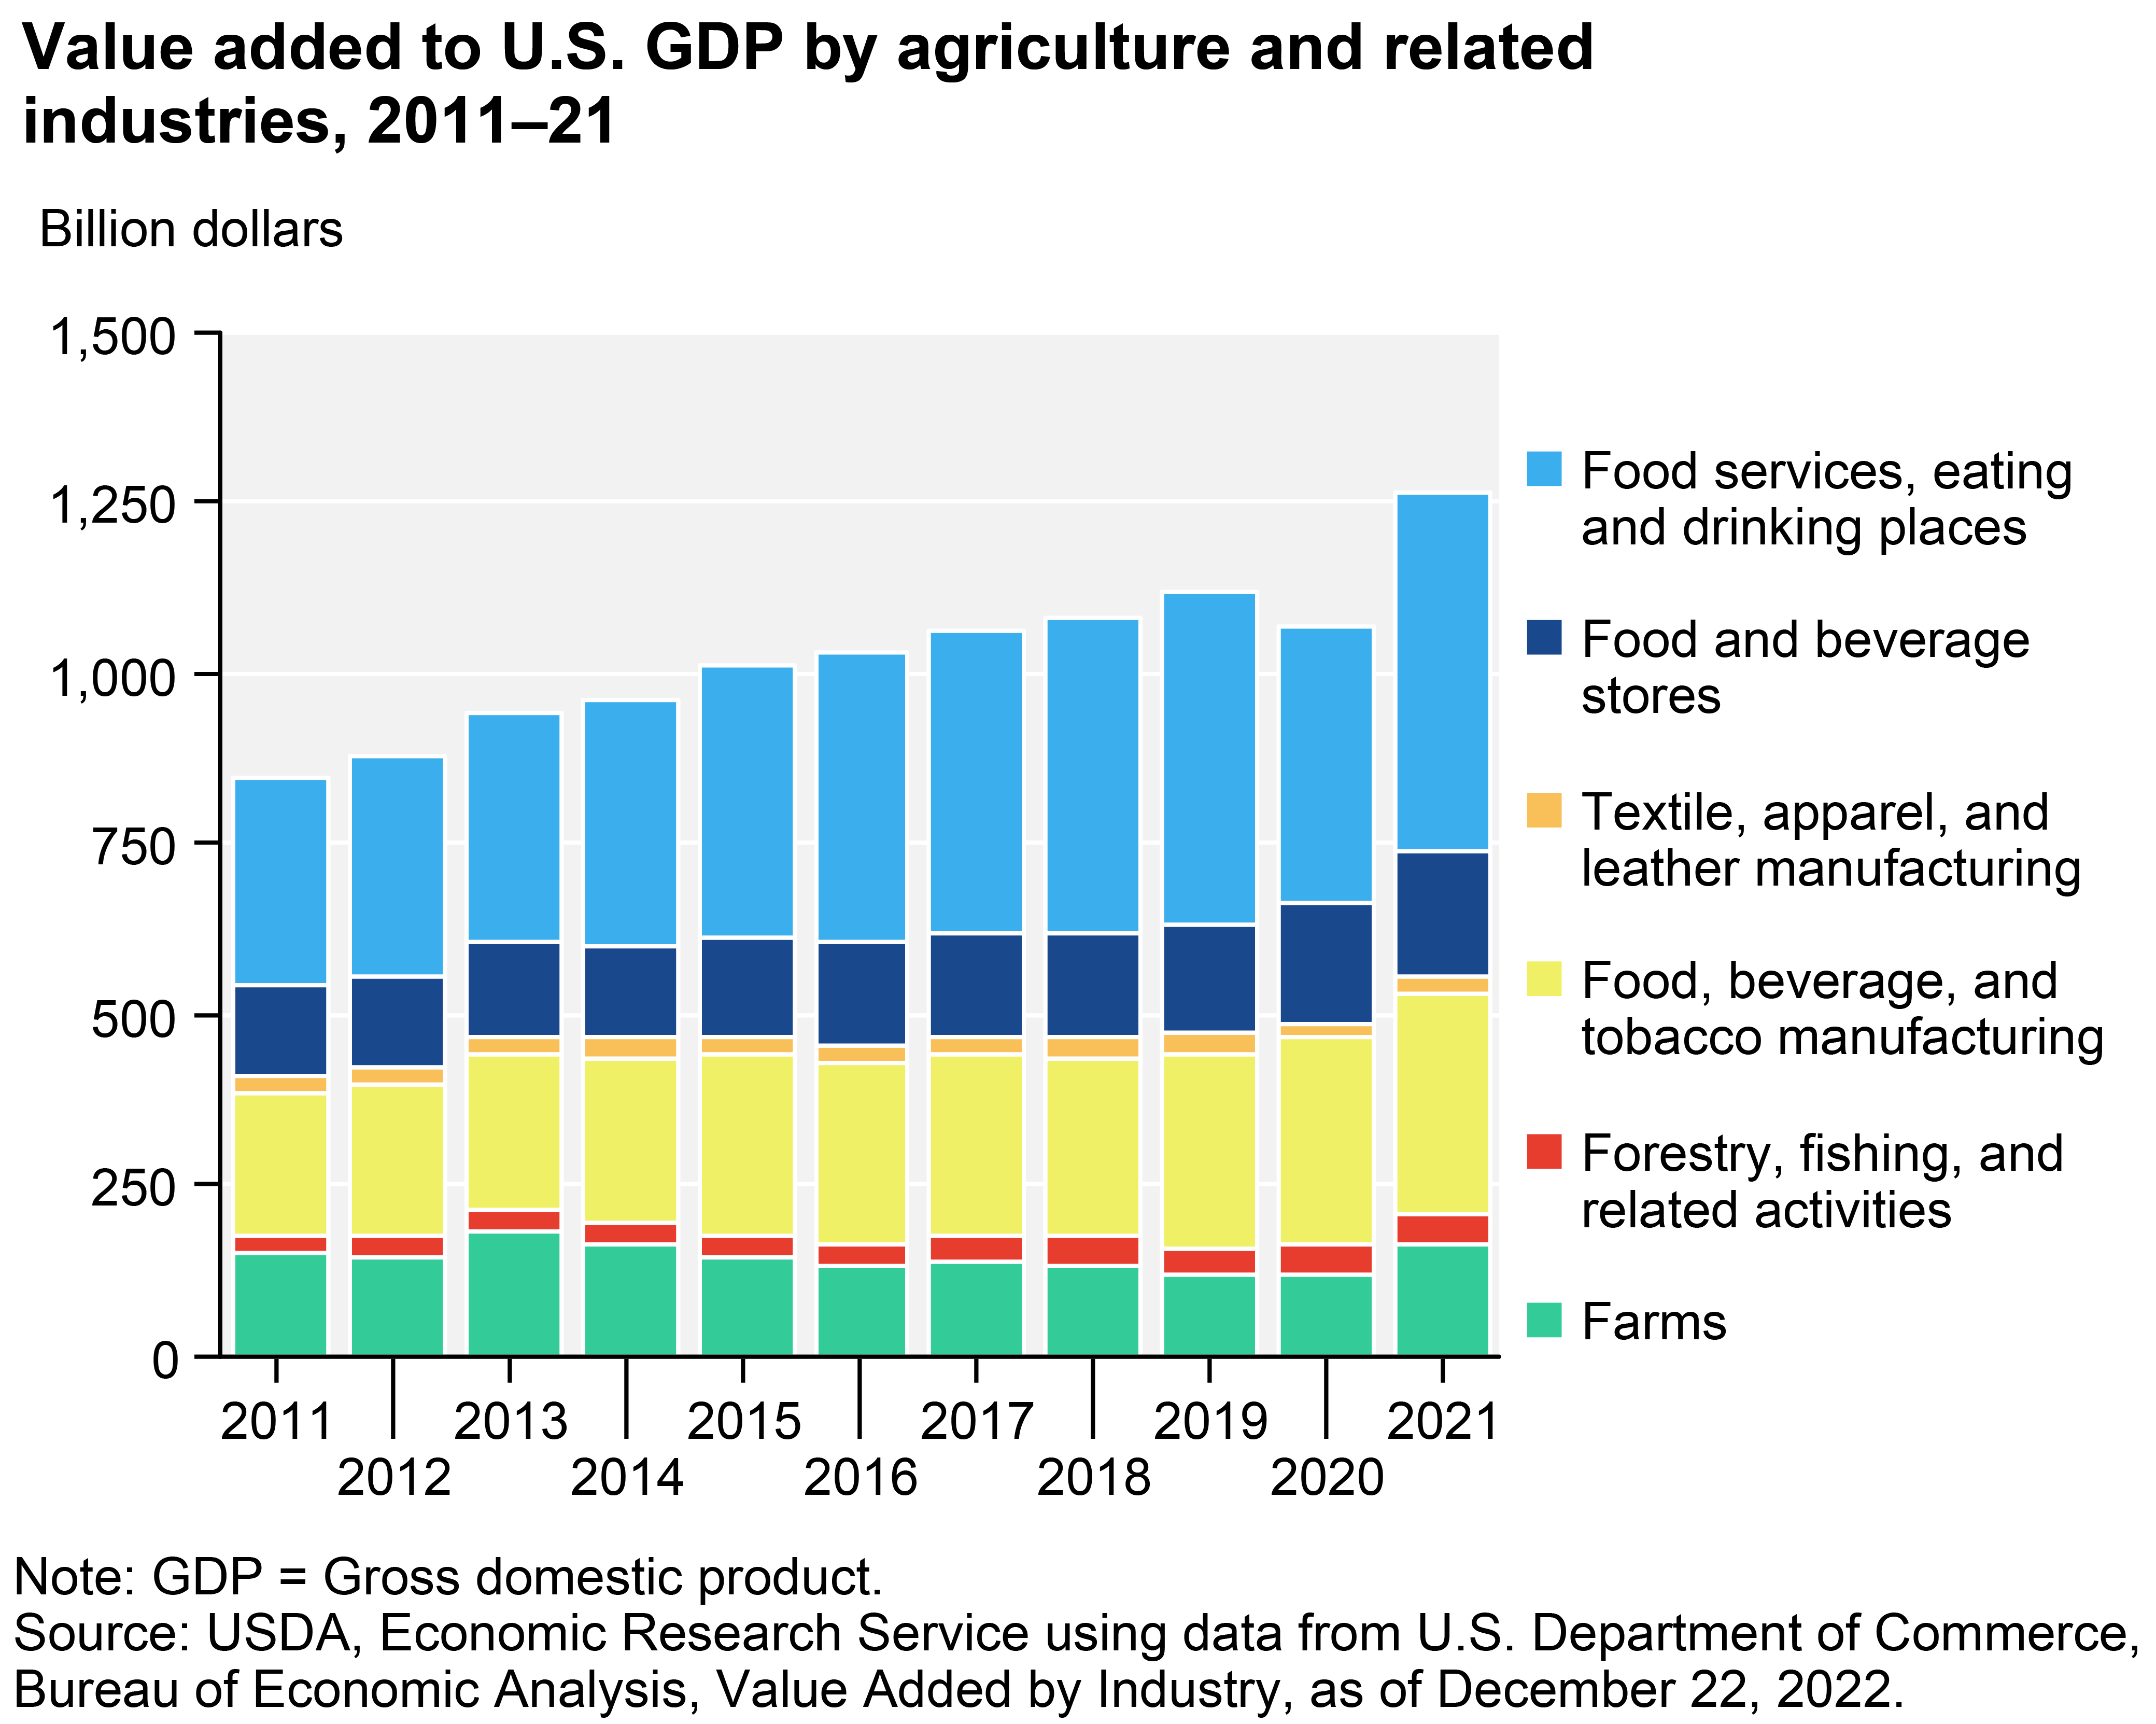
\includegraphics[width=0.85\linewidth]{Honors_Thesis/Figures/1.1.png}
\end{center}
\caption{Chart displaying the value added to U.S. GDP by Agriculture and related industries, 2011-21. Farms alone exceed \$150 billion annually.}
\label{fig:1.1}
\end{figure}

To account for rising number of pests and invasive species over the past century, farmers have increased their pesticide use to match, as seen in Fig \ref{fig:1.2} \cite{nehring_fernandez-cornejo_vialou_martin_wechsler_osteen}. Besides increased costs, the consequences of this rise in pesticide usage include unintentional environmental and human harm due to runoff and unintended targets \cite{aktar_sengupta_chowdhury_2009}. Another risk related to classic pesticide usage is the development of insecticide resistance through surviving insect populations and mutations \cite{gut_mcmanus_isaacs_schilder}. With this many risks associated with traditional pesticide use, adding more quantity can lead to diminishing returns on pesticide efficacy and even negative returns in extreme cases.

\begin{figure}[H]
\begin{center}
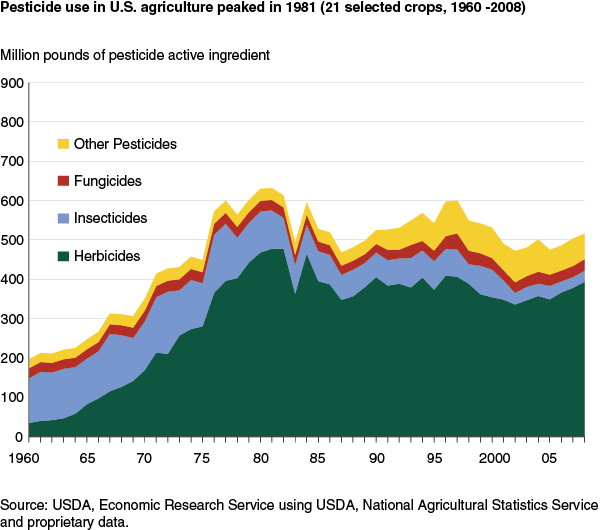
\includegraphics[width=0.9\linewidth]{Honors_Thesis/Figures/1.2.png}
\end{center}
\caption{Chart displaying the rise and fall of pesticide usage in the U.S. with a peak in 1981, 1960-2008.}
\label{fig:1.2}
\end{figure}

To combat the rise in pesticides we see in Fig \ref{fig:1.2} due to classic pest control methodologies, farmers began planting new pest-resistant strains of crops and implemented Integrated Pest Management (IPM). IPM is a pest control strategy that prioritizes long-term prevention through environmentally considerate methods. These methods include manipulating the pests' habitat, replacing possibly outdated practices by the farmer, planting resistant crop varieties, etc. Though there are many different IPM practices, all IPM programs contain the same six general components \cite{ipm}:

\begin{displayquote}
\begin{enumerate}
   \item Pest identification
   \item Monitoring and assessing pest numbers and damage
   \item Guidelines for when management action is needed
   \item Preventing pest problems
   \item Using a combination of biological, cultural, physical/mechanical and chemical management tools
   \item After action is taken, assessing the effect of pest management 
\end{enumerate}
\end{displayquote}

IPM is becoming increasingly adopted among farmers to reduce costs and yield losses. A concise version of an IPM is illustrated in Fig \ref{fig:1.3} \cite{hardy_lesher_olson_2021}. The limitation of many IPMs is their labor constraints, as the identification and monitoring of pests require consistent manual sampling, inspection, and expertise regarding insects \cite{zehnder_2009}. A novel system combining modern hardware and software has been developed to address these challenges to create a consistent and efficient pest identification and monitoring method.

\begin{figure}[H]
\begin{center}
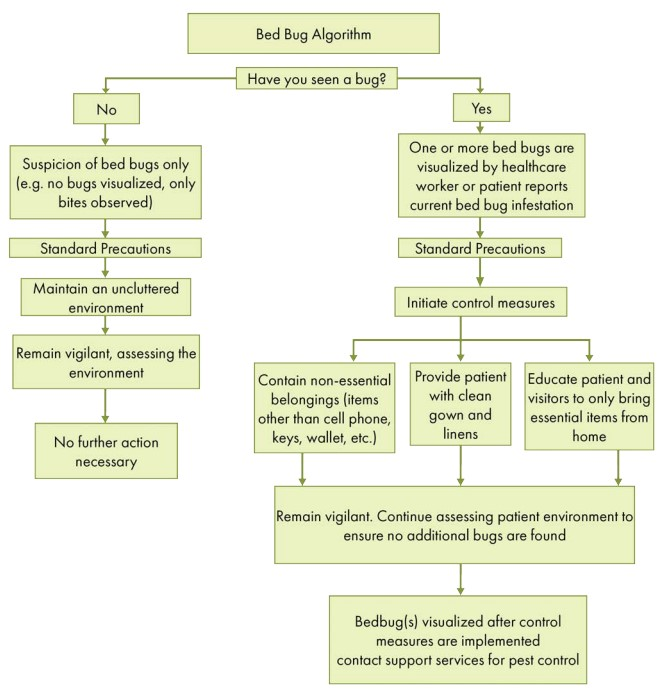
\includegraphics[width=0.95\linewidth]{Honors_Thesis/Figures/1.3.jpg}
\end{center}
\caption{Bed Bug Algorithm: small-scale Integrated Pest Management (IPM) plan.}
\label{fig:1.3}
\end{figure}

Integrating an on-site camera system running an insect detection and classification model with a user-facing application can revolutionize farmers' management of pests. By leveraging Artificial Intelligence, farmers can take informed action and track pest numbers in real-time, thereby improving the sustainability of IPM plans and increasing the efficiency of pest management. Furthermore, the system is complemented by the integration of an additional AI model that is used to emulate an agriculture expert: OpenAI's GPT-3.5. This feature provides farmers with personalized recommendations based on their unique farm conditions, allowing for faster and more effective pest control strategies. This innovative approach can potentially reduce the use of harmful pesticides and improve crop yields by a significant amount.
